\documentclass[dvipdfmx]{beamer}
\usepackage{bxdpx-beamer}% dvipdfmxなので必要
\usepackage{pxjahyper}% 日本語で'しおり'したい
%\usepackage{etex}
%\usetheme{Warsaw}
\usetheme{Malmoe}
%\usetheme{AnnArbor}
%\usetheme{Hannover}
%\usetheme{Bergen}
%\usetheme{Berlin}
%\usetheme{Singapore}
%\usetheme{Montpellier}
%\usetheme{Pittsburgh}
\usepackage{graphicx}
\usepackage{latexsym,amssymb}
\usepackage{amsthm}
%\usepackage{epsbox}
%\usepackage{multirow}
\usepackage{fancybox}
\usepackage{ascmac}
\usepackage{fancyvrb}
%\usepackage{listings}
\usepackage{tabularx}
\usepackage{tikz}
\usetikzlibrary{calc,shapes}
%\usepackage{pstricks,pst-node,pst-tree}
%\usepackage{multimedia}
%\usepackage{pstricks,pst-node,pst-tree}
%\usepackage{pst-all}
%\include{prooftree}
%\lstloadlanguages{pascal}
\usepackage{mathrsfs}

\renewcommand{\kanjifamilydefault}{\gtdefault}
\renewcommand{\familydefault}{\sfdefault}

\graphicspath{{figs261117/}}

%\include{cmacros}

\newcommand{\greentext}[1]{{\color[rgb]{0,0.5,0}{#1}}}
\newcommand{\redtext}[1]{{\color[rgb]{0.8,0,0}{#1}}}
\newcommand{\bluetext}[1]{{\color[rgb]{0,0,0.8}{#1}}}

\newcommand{\tuple}[1]{\langle{#1}\rangle}

\newcommand{\First}{\mathsf{First}_1}
\newcommand{\Follow}{\mathsf{Follow}_1}

%%pdt simulation

\newcommand{\pdtline}[6]{%
    \uncover<#6->{
    \node at (${#5}*(0,-.3)+(0,.3)$) {$\vdash$};%
    \node at (${#5}*(0,-.3)+(1.5,.3)$) {\parbox{12em}{(#1,}};%
    \node at (${#5}*(0,-.3)+(4.5,.3)$) {\parbox{10em}{#2,}};%
    \node at (${#5}*(0,-.3)+(5.7,.3)$) {\parbox{10em}{#3)}};%
    \node at (${#5}*(0,-.3)+(8,.3)$) {\parbox{20em}{#4}};%
    }
}

\newcommand{\initpdtline}[6]{%
    \uncover<#6->{
    \node at (${#5}*(0,-.3)+(1.5,.3)$) {\parbox{12em}{(#1,}};%
    \node at (${#5}*(0,-.3)+(4.5,.3)$) {\parbox{10em}{#2,}};%
    \node at (${#5}*(0,-.3)+(5.7,.3)$) {\parbox{10em}{#3)}};%
    \node at (${#5}*(0,-.3)+(8,.3)$) {\parbox{20em}{#4}};%
    }
}

\newtheorem{Def}{定義}
\newtheorem{Lem}{補題}
\newtheorem{Thm}{定理}
\newtheorem{Prop}{命題}

\newenvironment{CustomDef}[2]{%
  \par\medskip\noindent
  \textbf{定義 #1}({#2})\quad\ignorespaces
}{%
  \par\medskip
}


\definecolor{lightlightgrey}{rgb}{0.95,0.95,0.95}

\newcommand{\vdom}{\underline{\gg}}
\newcommand{\svdom}{\gg}
\newcommand{\domll}{\underline{\ll}}
\newcommand{\domv}[1]{\mathsf{dom}({#1})}
\newcommand{\idomv}[1]{\mathsf{idom}({#1})}

%\newcommand{\greentext}[1]{{\color[rgb]{0,0.5,0}{#1}}}
%\newcommand{\redtext}[1]{{\color[rgb]{0.8,0,0}{#1}}}

\newcommand{\lecturedate}{2026/11/17}

\cornersize{0.25}

\setbeamertemplate{frametitle}[default][center]
\setbeamertemplate{footline}{\hfill
コンパイラ\quad\lecturedate
\hfill\insertframenumber/\inserttotalframenumber\hspace*{1zw}}
\newcounter{coffee}
\setbeamercovered{transparent=10}
\title{コンパイラ(13)}
\date{\lecturedate}
\begin{document}
\begin{frame}
  \frametitle{SSA形式に対する最適化}
  SSA形式：データフロー解析ずみのプログラム\\[2zw]

  \greentext{構文的にフローが表現されている}
  $\Rightarrow$
  \redtext{最適化を効果的に適用できる}：
  \greentext{更新のチェックが不要}

  例：DAGの構成が容易

  \vspace*{1zw}

  \begin{itemize}
    \item 不用コードの削除
    \item 定数伝播
    \item コピー伝播
    \item 共通部分式の削除
    \item ループ不変コードの移動
  \end{itemize}
\end{frame}

\begin{frame}
  \frametitle{SSA最適化例 [佐々:06]}

  \only<1>{
    \begin{center}
      \begin{tabular}{ccc}
        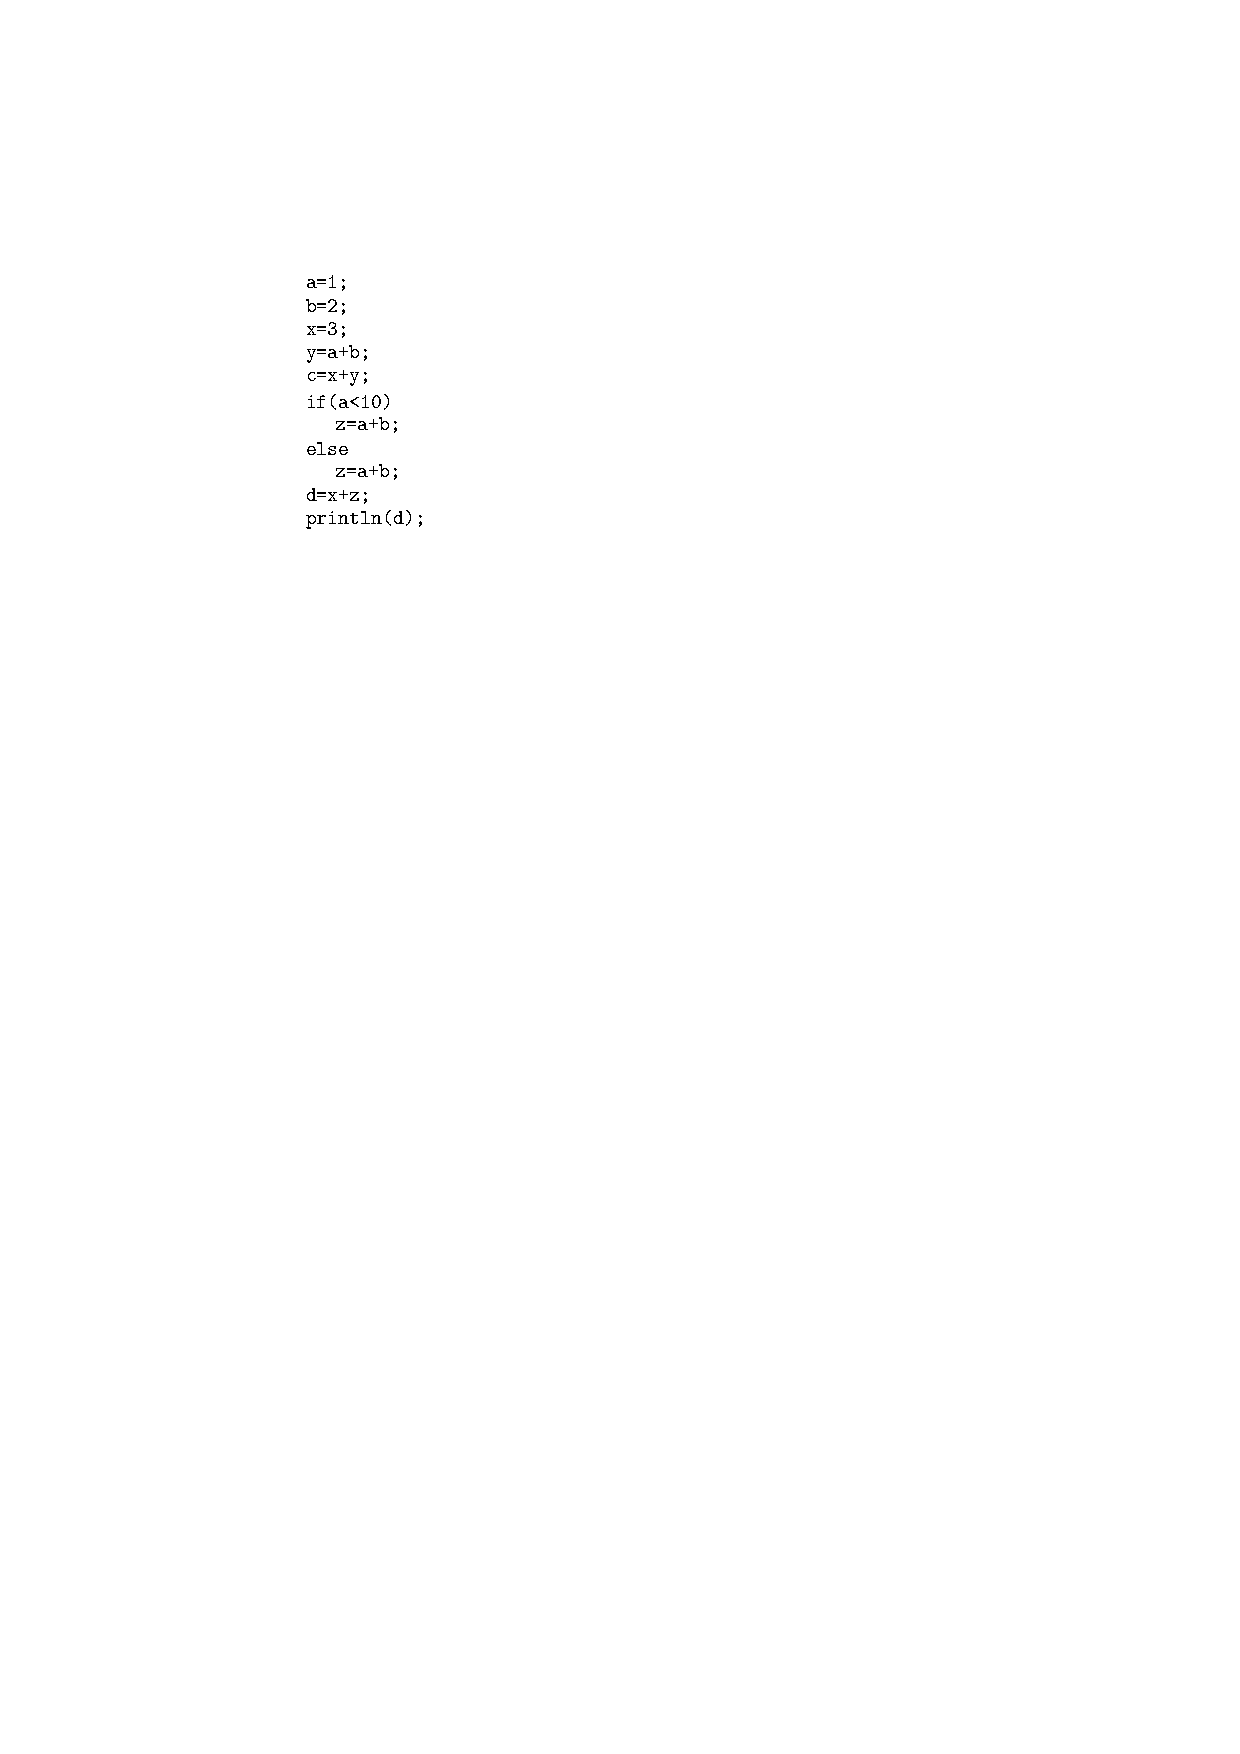
\includegraphics{ssasrc01.pdf}
         & $\Rightarrow$ &
        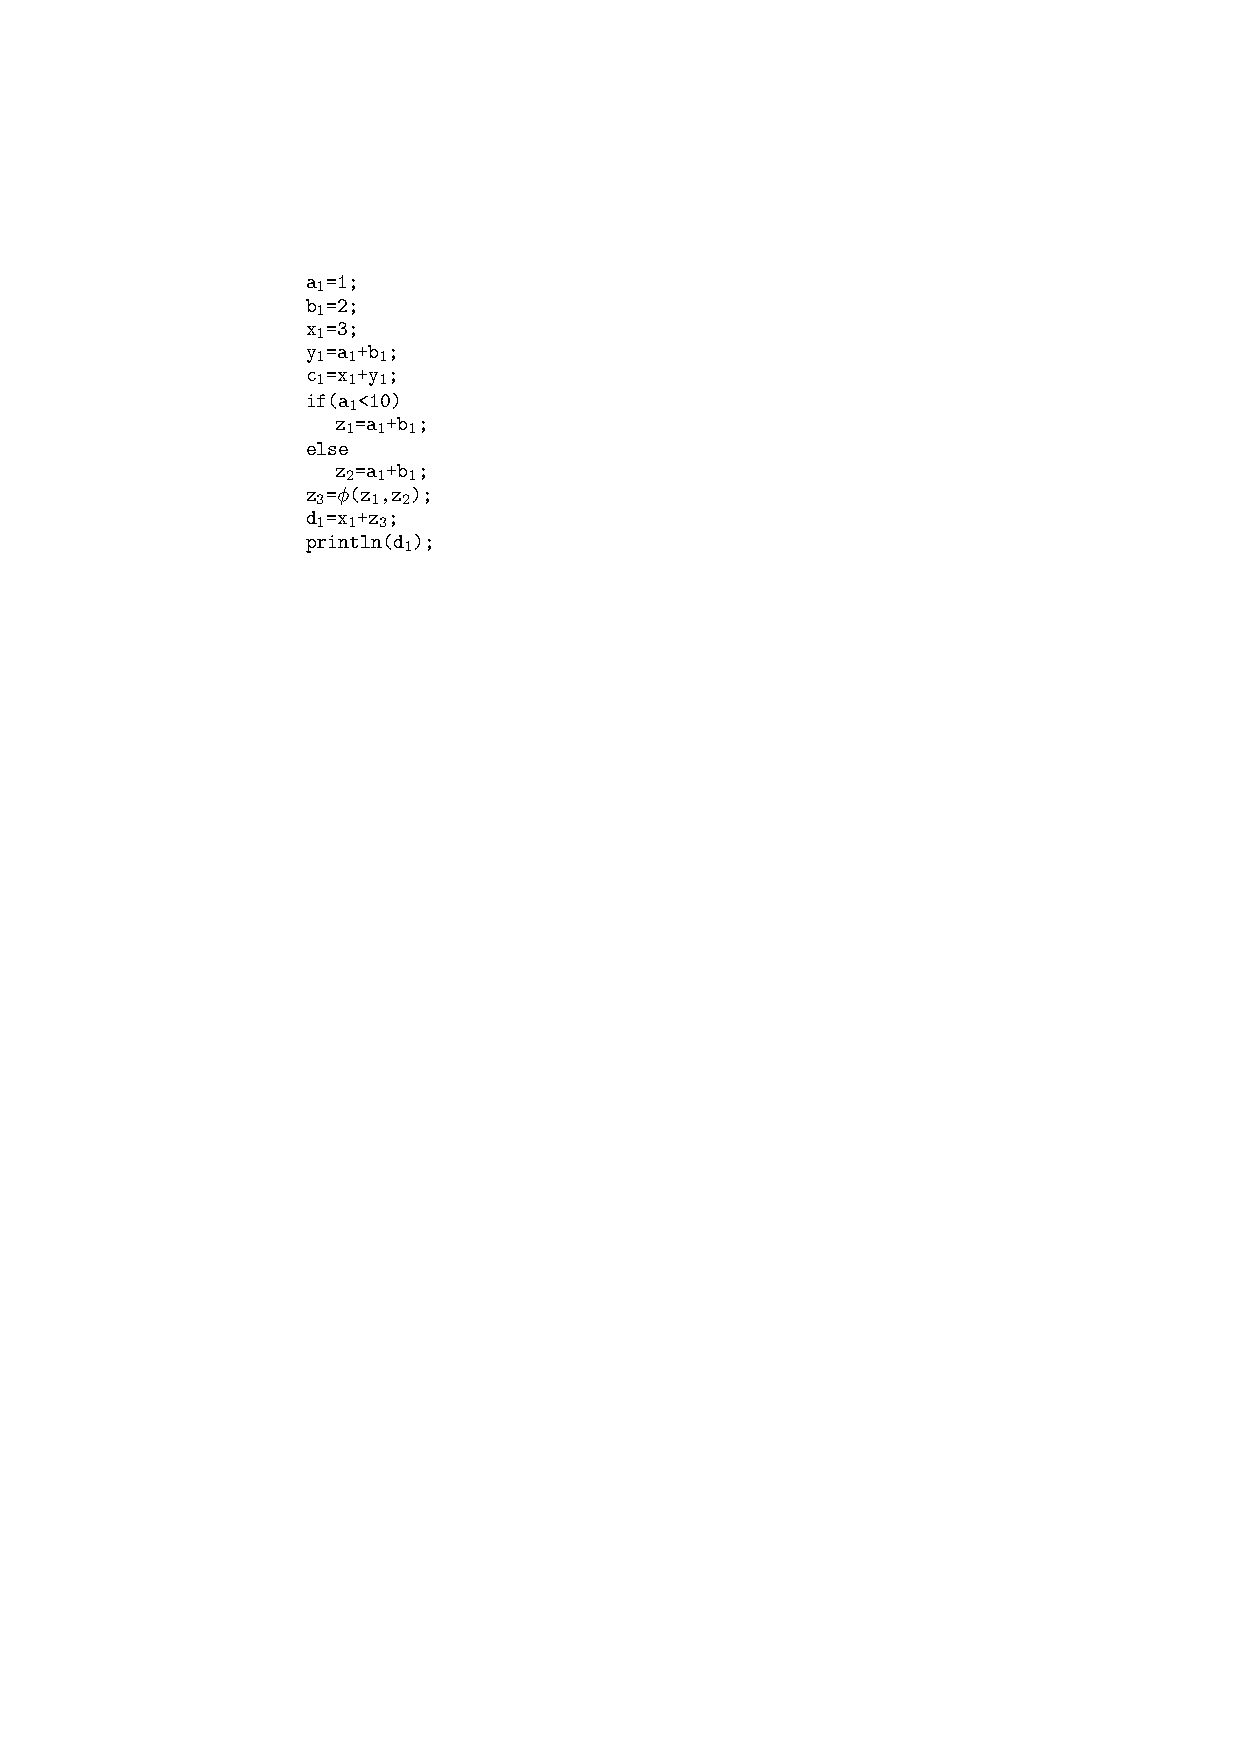
\includegraphics{ssasrc02.pdf}
        \\[1zw]
        \multicolumn{3}{c}{\greentext{SSA形式へ変換}}
      \end{tabular}
    \end{center}
  }

  \only<2>{
    \begin{center}
      \begin{tabular}{ccc}
        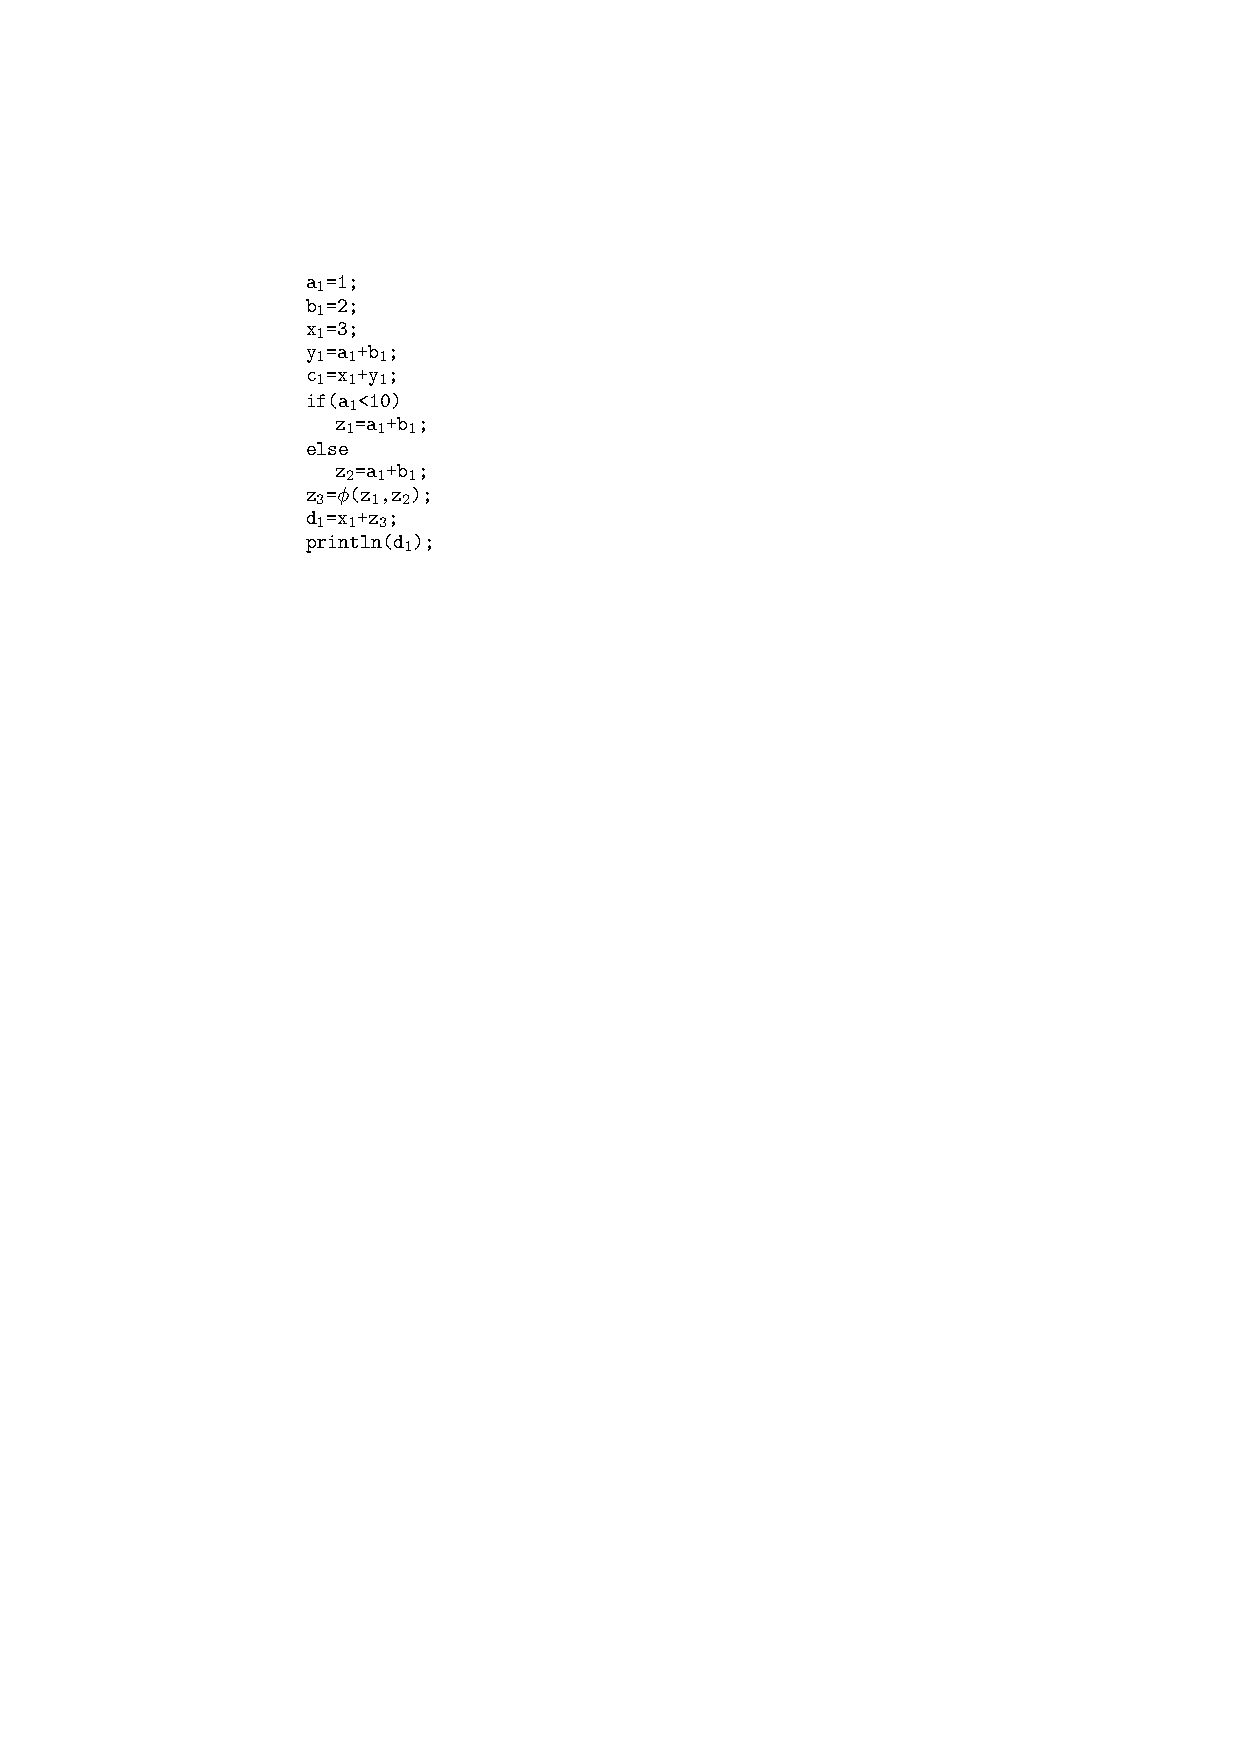
\includegraphics{ssasrc02.pdf}
         & \hspace*{1zw}$\Rightarrow$\hspace*{1zw} &
        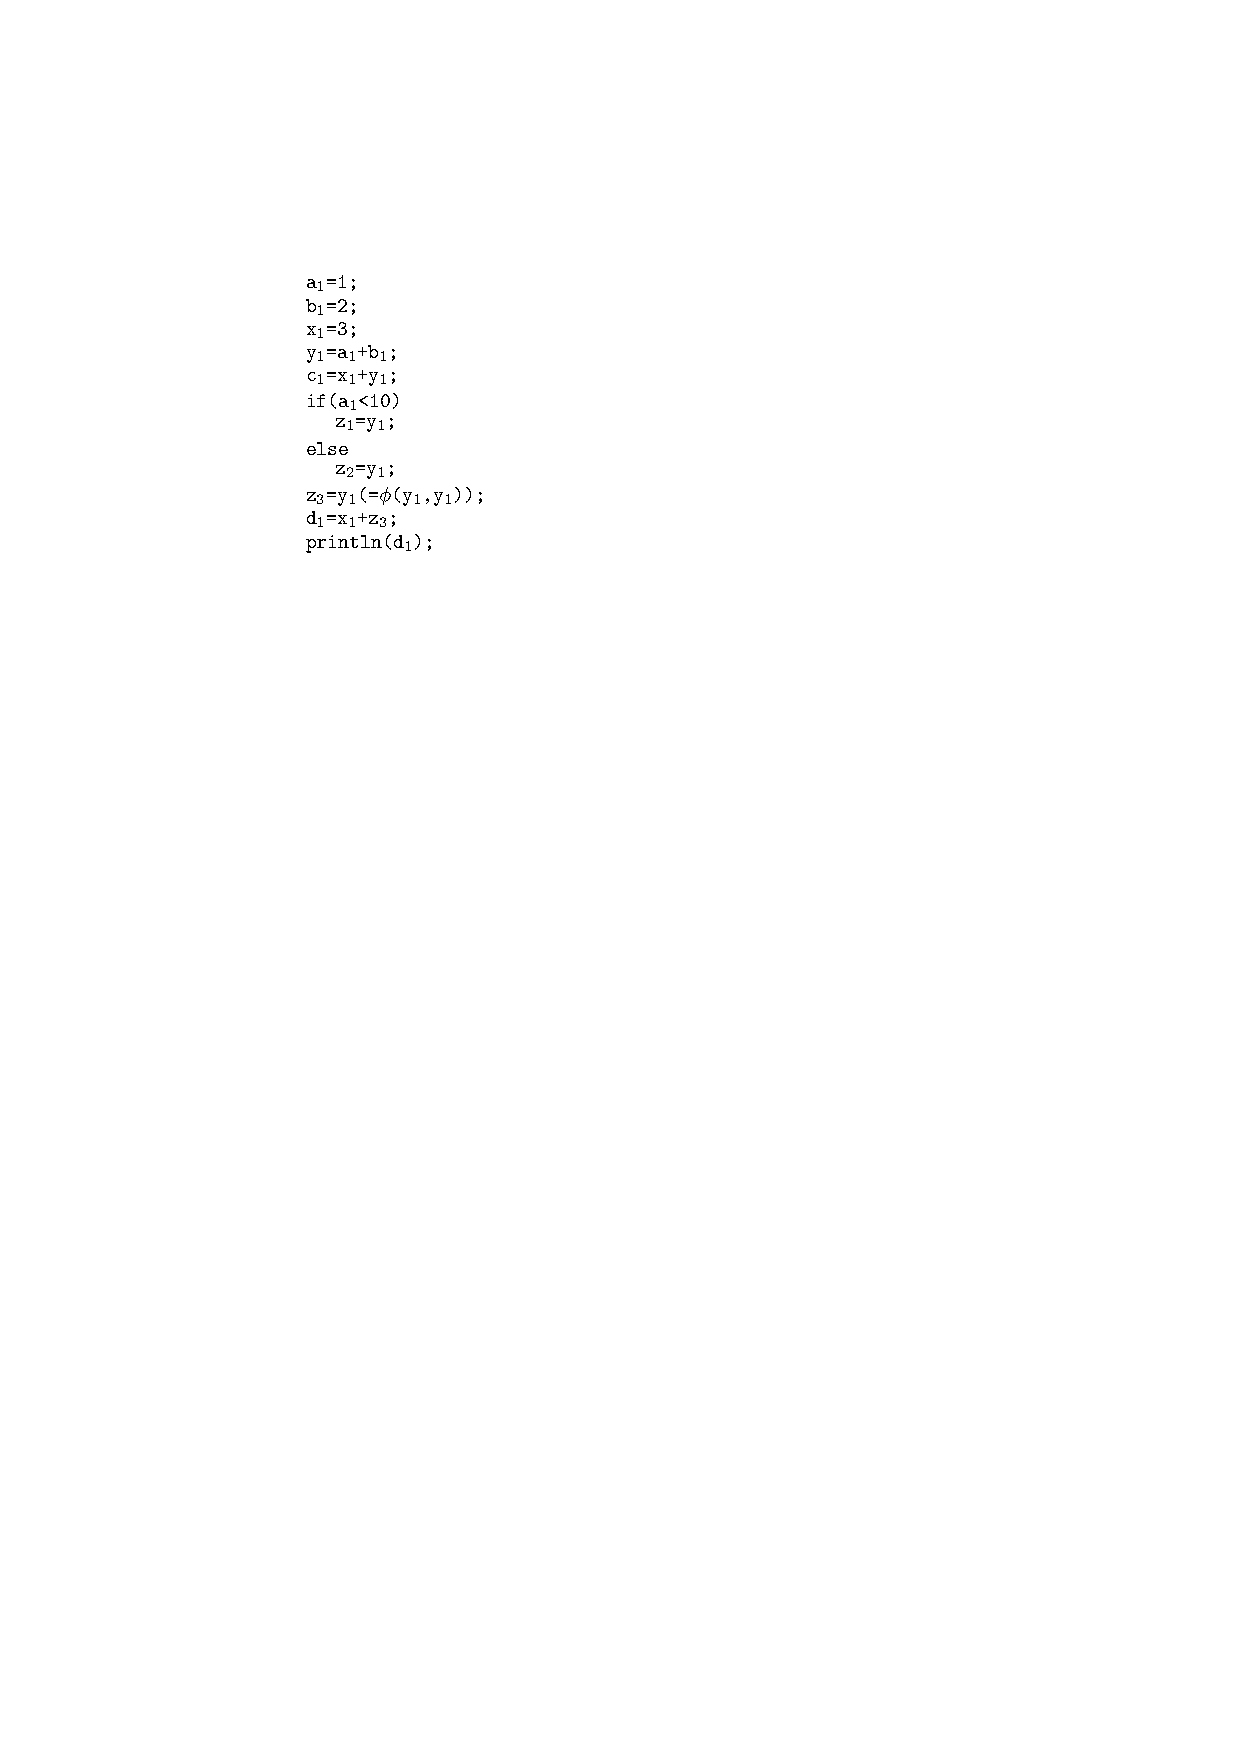
\includegraphics{ssasrc03.pdf}               \\[1zw]
        \multicolumn{3}{c}{\greentext{共通部分式除去}}
      \end{tabular}
    \end{center}
  }

  \only<3>{
    \begin{center}
      \begin{tabular}{ccc}
        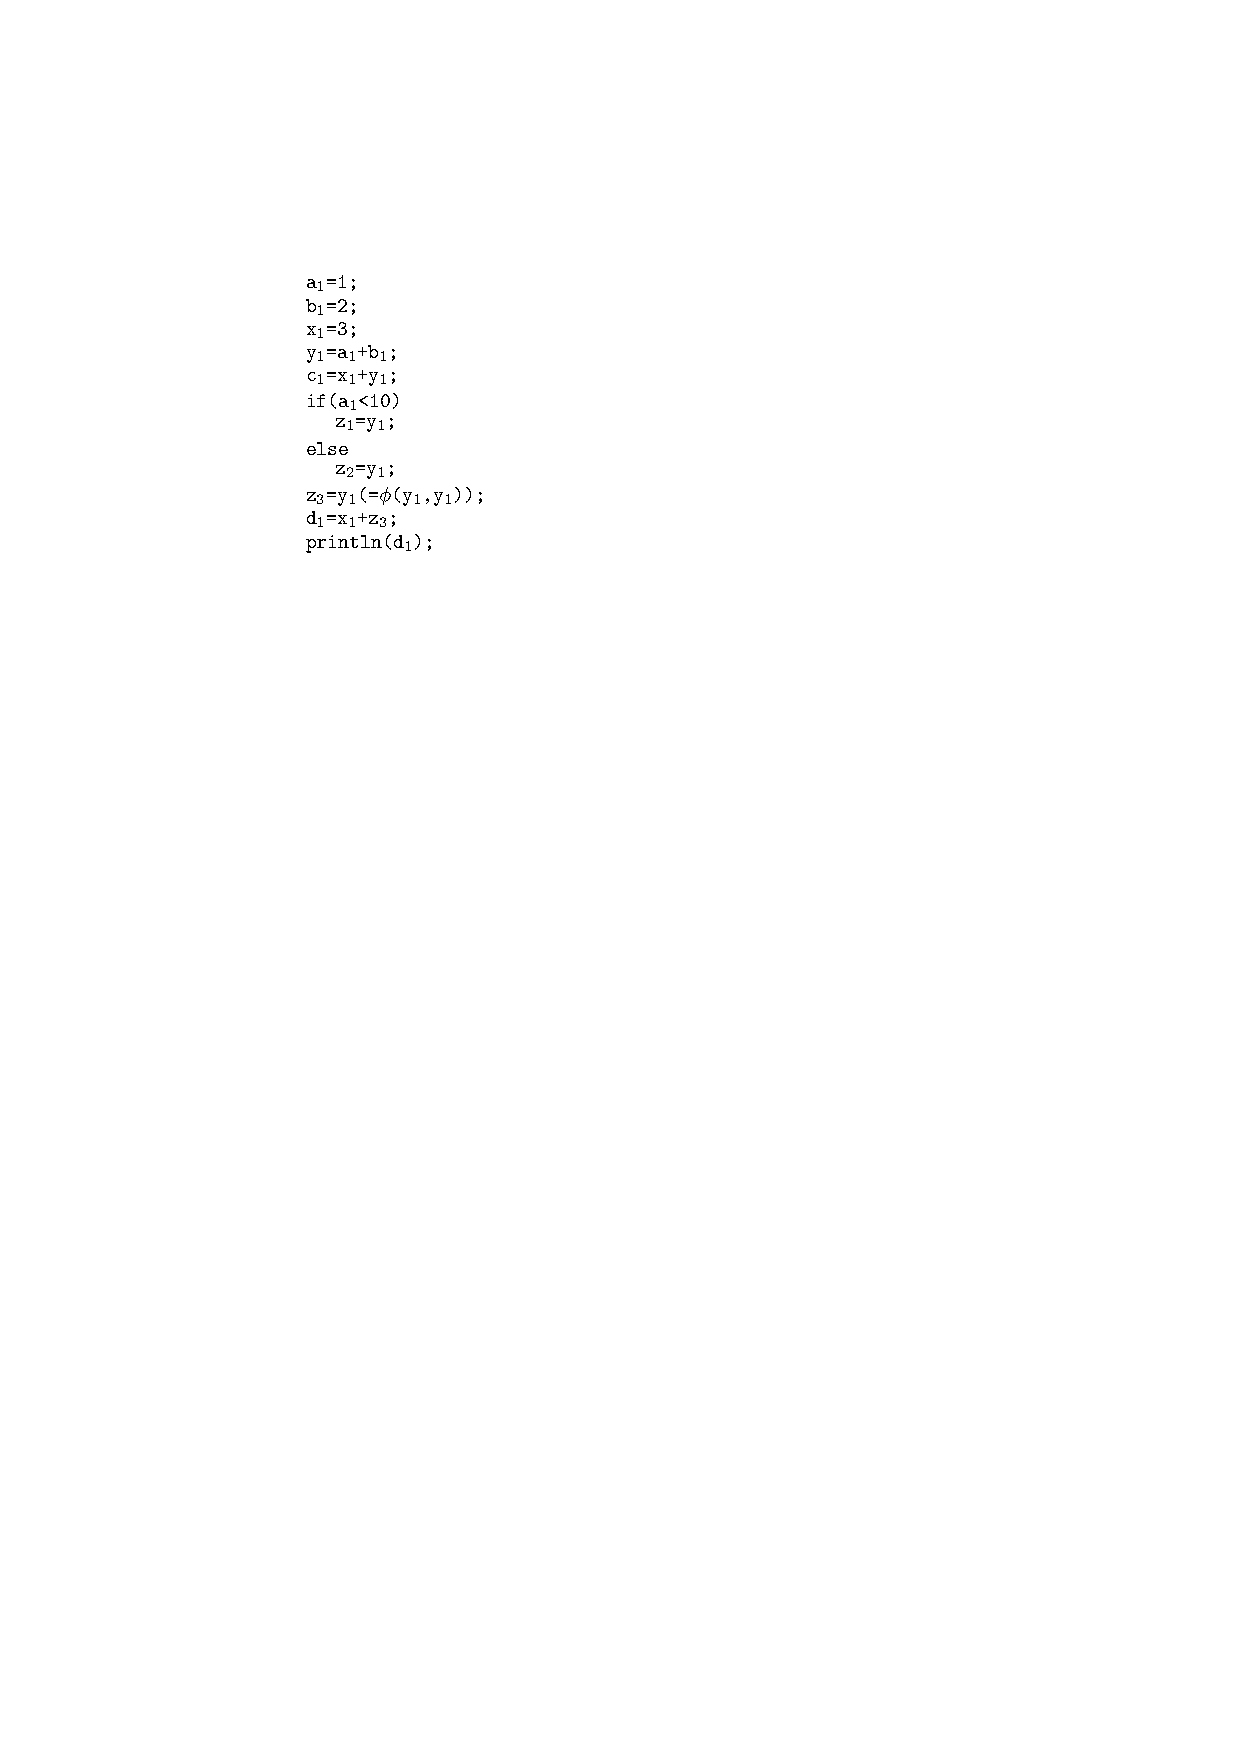
\includegraphics{ssasrc03.pdf}
         & \hspace*{1zw}$\Rightarrow$\hspace*{1zw} &
        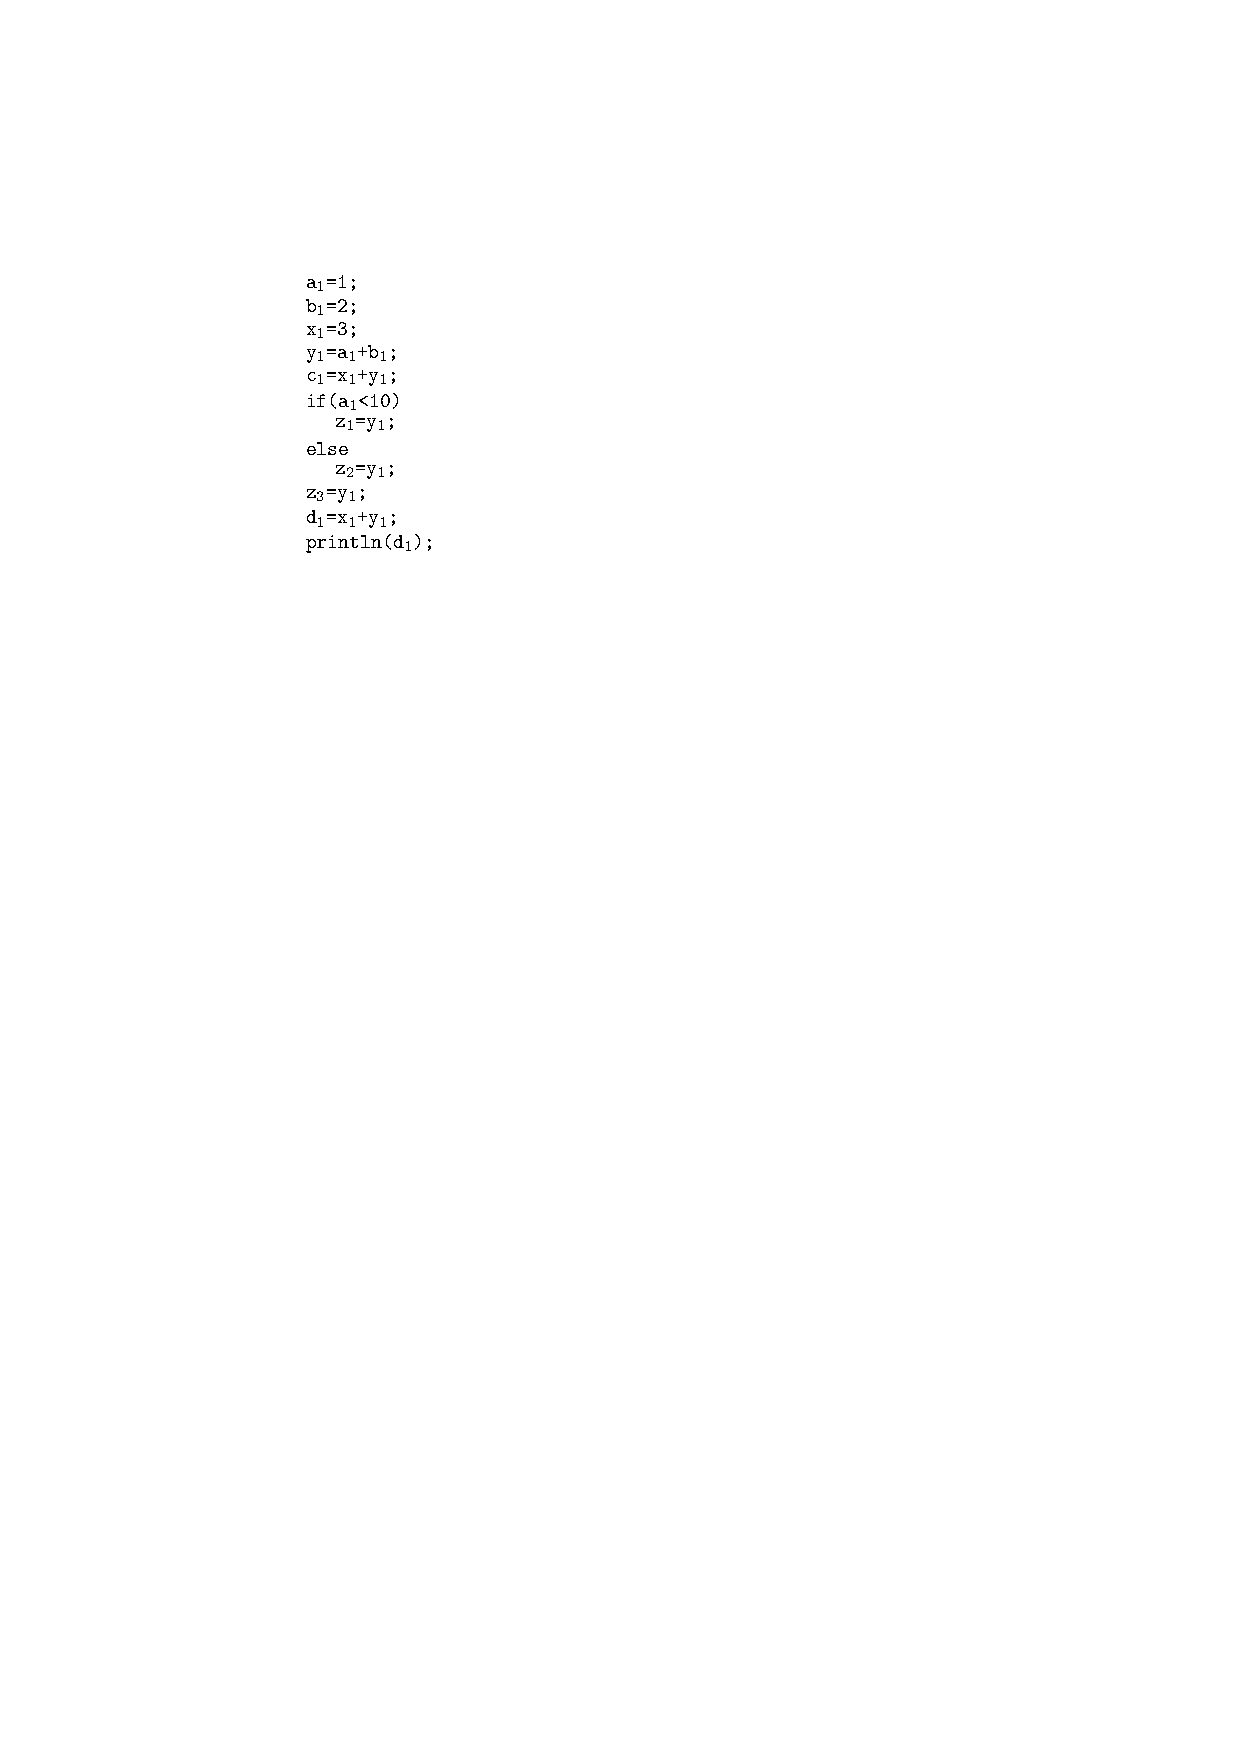
\includegraphics{ssasrc04.pdf}               \\[1zw]
        \multicolumn{3}{c}{\greentext{コピー伝播}}
      \end{tabular}
    \end{center}
  }

  \only<4>{
    \begin{center}
      \begin{center}
        \begin{tabular}{ccc}
          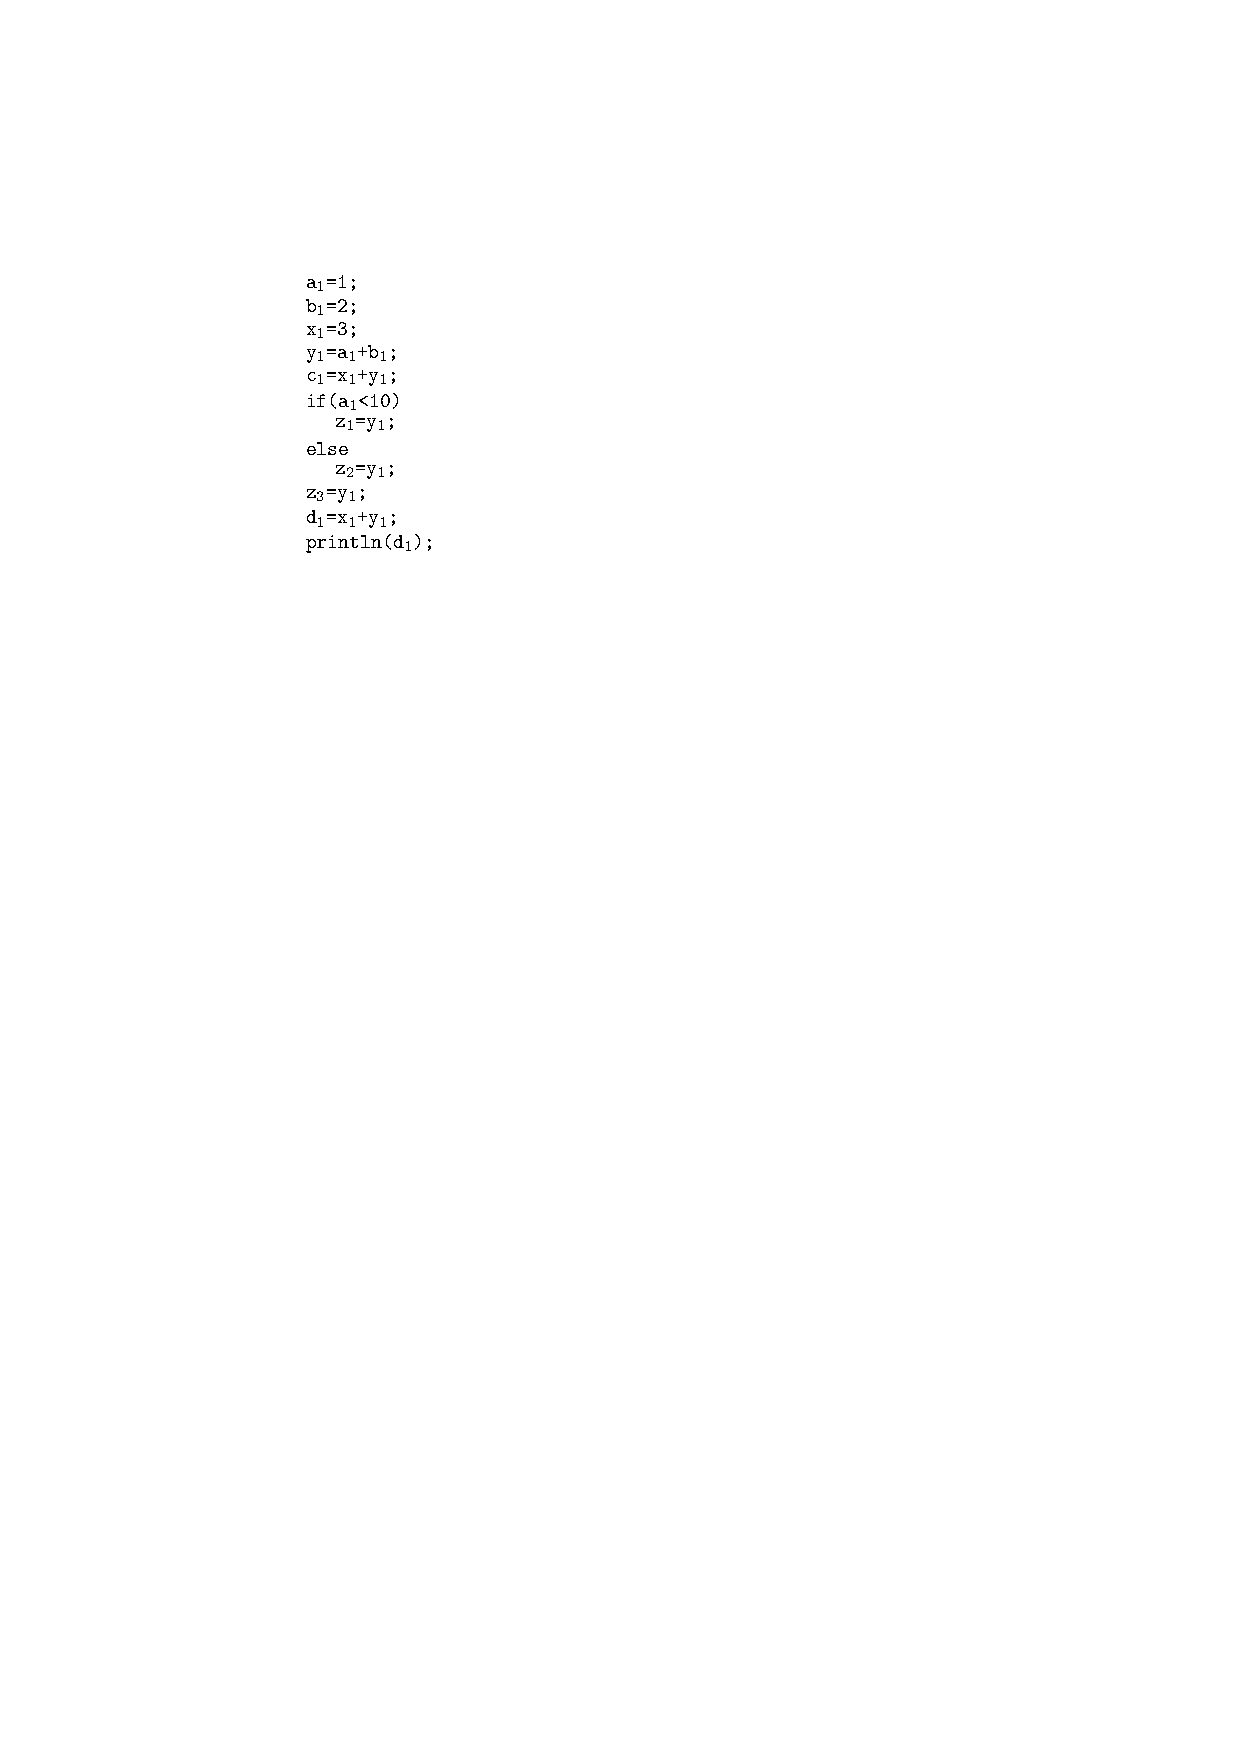
\includegraphics{ssasrc04.pdf}
           & \hspace*{1zw}$\Rightarrow$\hspace*{1zw} &
          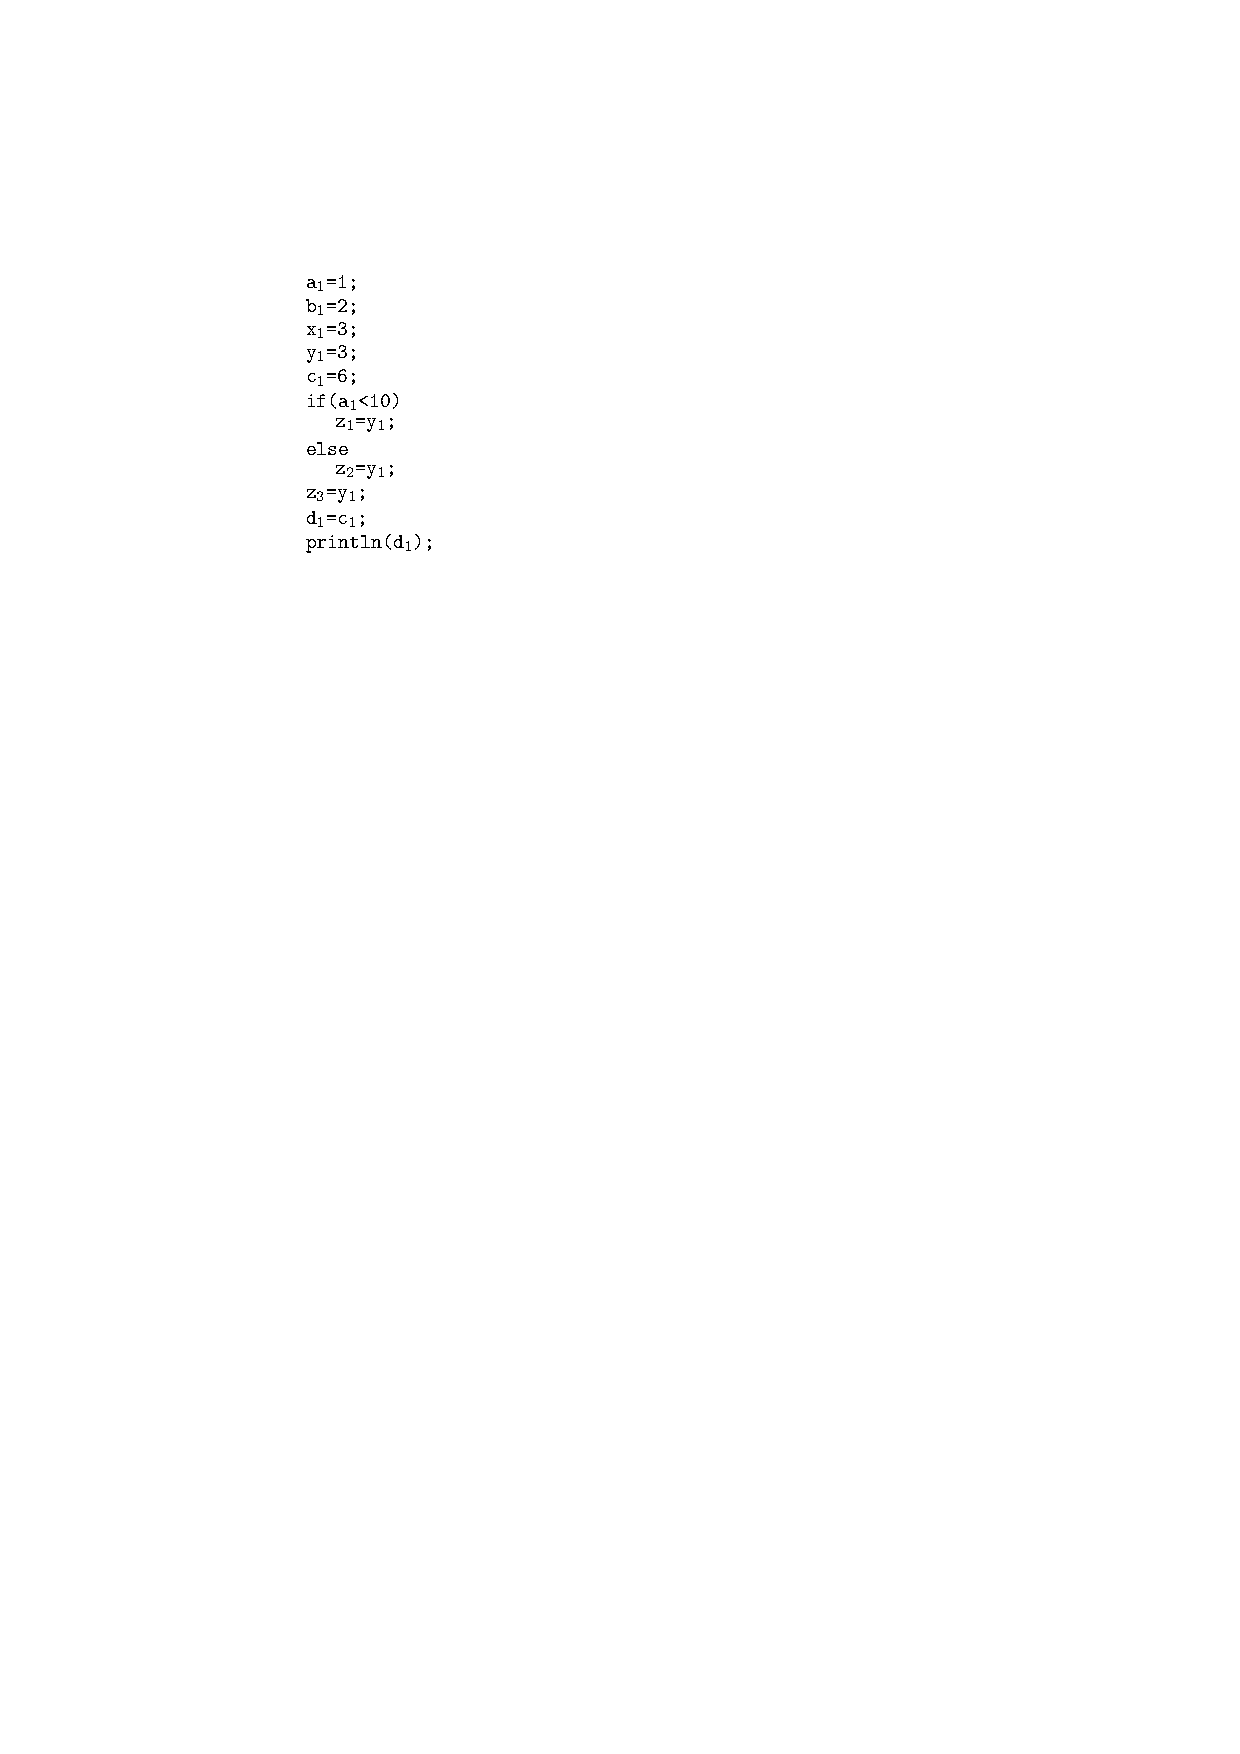
\includegraphics{ssasrc05.pdf}               \\[1zw]
          \multicolumn{3}{c}{\greentext{共通部分式除去、定数伝播}}
        \end{tabular}
      \end{center}
    \end{center}
  }

  \only<5>{
    \begin{center}
      \begin{tabular}{ccc}
        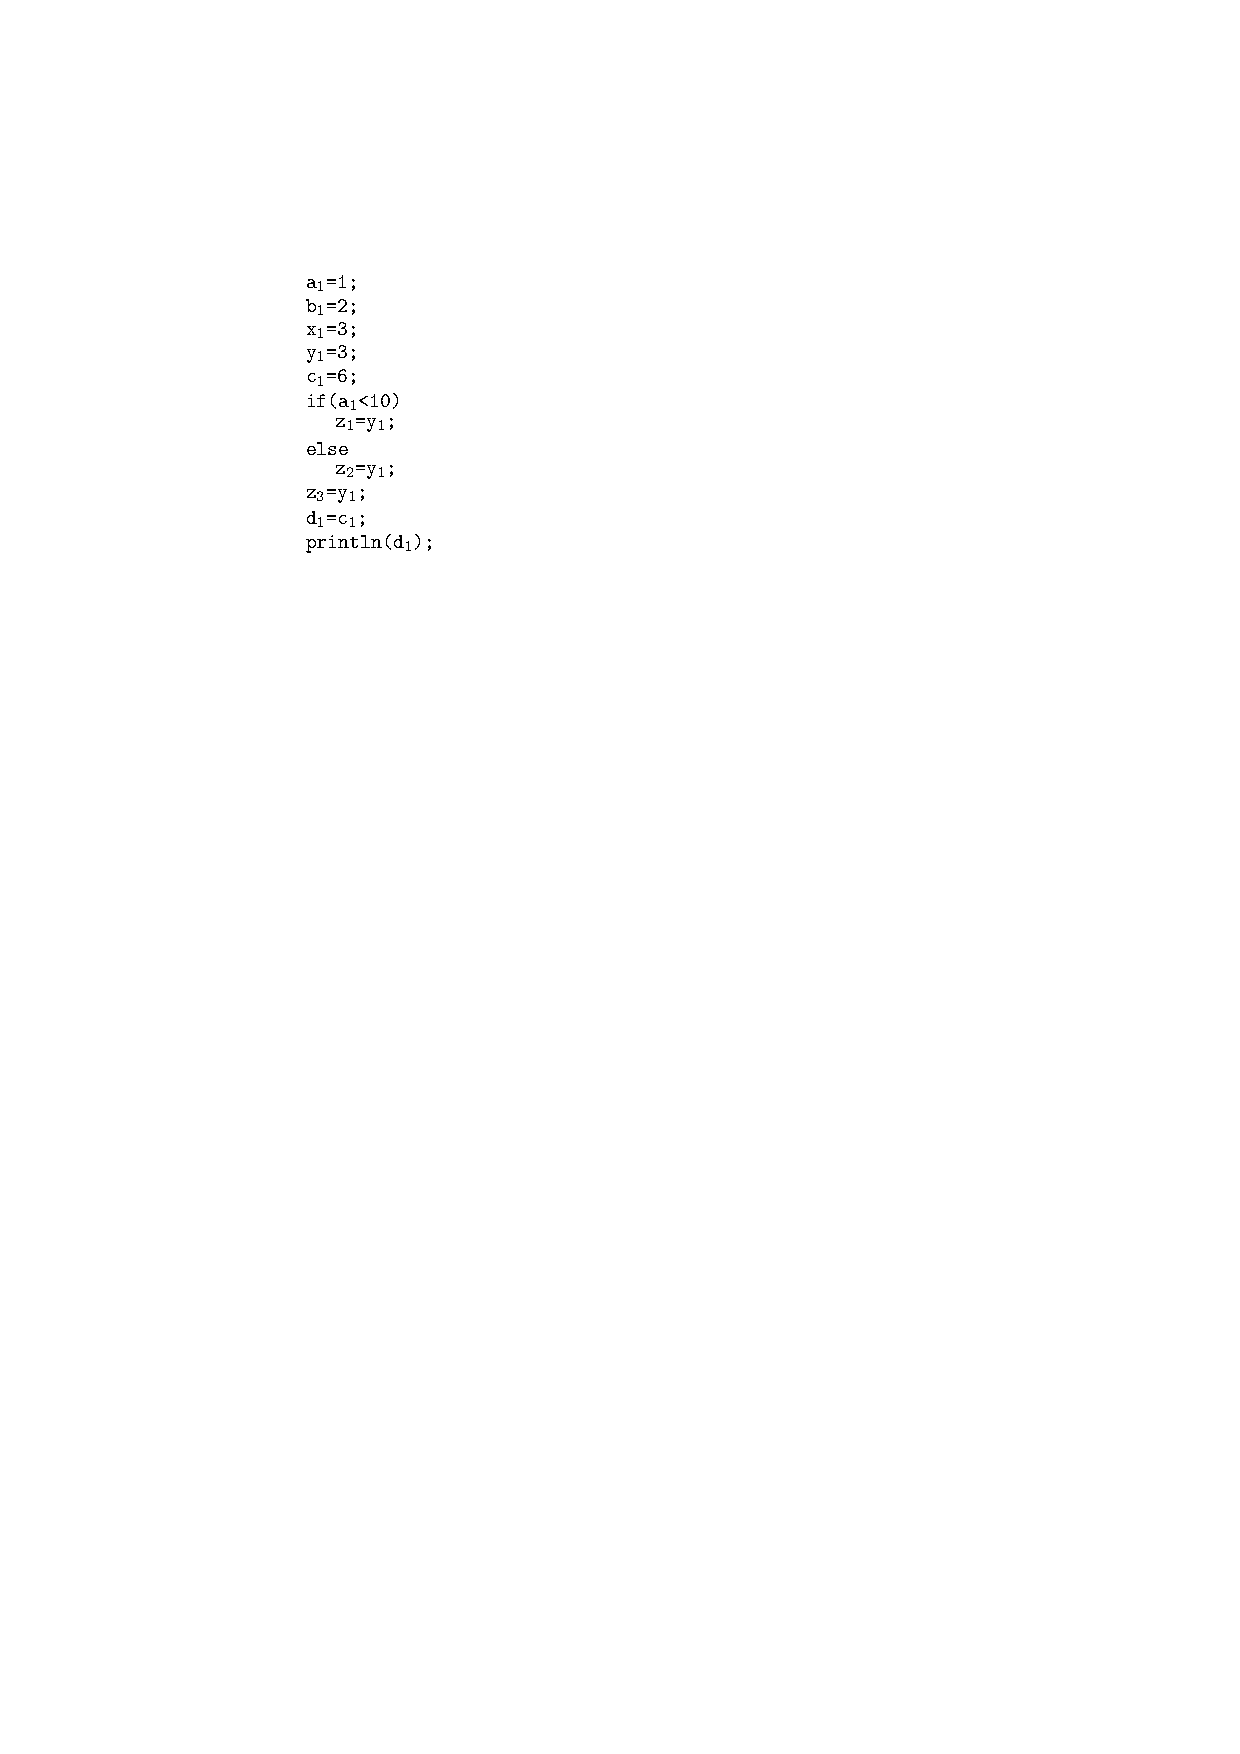
\includegraphics{ssasrc05.pdf}
         & \hspace*{1zw}$\Rightarrow$\hspace*{1zw} &
        
\includegraphics{ssasrc06.pdf}               \\[1zw]
        \multicolumn{3}{c}{\greentext{コピー伝播、定数伝播、恒等式}}
      \end{tabular}
    \end{center}
  }

\end{frame}

\begin{frame}
  \frametitle{最適化の条件}

  最適化を行うときに支配関係を壊さないようにする。

    \begin{center}
        \begin{tabular}{ccc}
            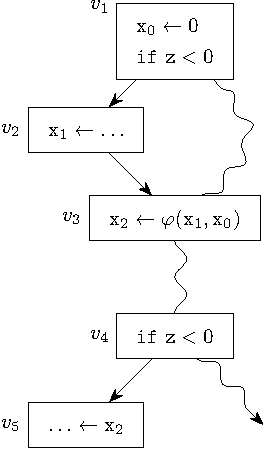
\includegraphics[scale=0.6]{SSA-dominance-break-crop.pdf}
                    &  &
            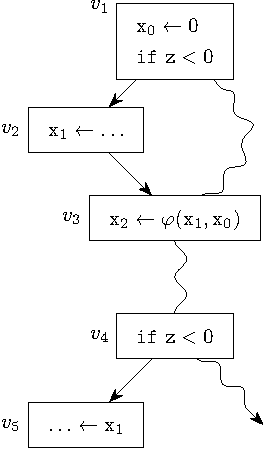
\includegraphics[scale=0.6]{SSA-dominance-break-after-crop.pdf} \\
            (a)最適化前 &  & (b)最適化後
        \end{tabular}
    \end{center}

  $z<0$の評価は同じ方向にしかブランチしない\\
  $\Rightarrow$ $z<0$ならば3の$\phi$関数はいつも$x_1$を$x_2$へ代入\\
  5において$z<0$で、$x_1$を参照に用いると支配関係が壊れる\\[5pt]
  %(支配関係を壊すと一般にはデータフローが保証されない)\\
  厳密SSA形式：\redtext{定義が一意的＋支配関係}
  %\greentext{静的と動的のギャップを$\phi$関数で埋めているため}
\end{frame}

\begin{frame}
  \frametitle{条件付き定数伝播[Tigerbook]}
  \begin{center}
    {\begin{tabularx}{.75\textwidth}{XXX}
      \multicolumn{1}{m{.35\textwidth}}{
      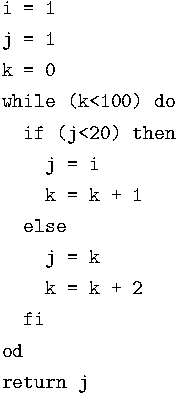
\includegraphics[height=.7\textheight]{prog-example-crop.pdf}
      }
      & \multicolumn{1}{m{2em}}{$\Rightarrow$} &
      \multicolumn{1}{m{.4\textwidth}}{
      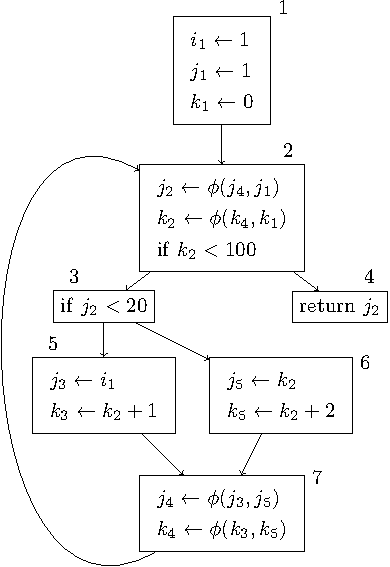
\includegraphics[height=.7\textheight]{SSA-prog-crop.pdf}
      }
     \end{tabularx}}
  \end{center}
  \centerline{\greentext{6のブロックは実行されるか？}}
\end{frame}

\begin{frame}
  \frametitle{アルゴリズム}
  {\scriptsize
  \begin{tabular}{l}
  $\mathcal{B}[n]=true$ならばブロック$n$は実行される可能性あり\\
  $\mathcal{V}[x]$ 定数$c$, 決まらない$\top$, 初期化されない$\bot$
  \end{tabular}}

  \vspace*{5pt}

  {\scriptsize\color[rgb]{0,0.5,0}
  $\phi(x_1,\ldots,x_n)$において，$x_i$のフロー元となる直近のブロックを$b_i$と書く．
  }

  \vspace*{5pt}

  {\scriptsize
  初期化：$\mathcal{B}[n]=false$ ($1\leq n\leq N$), 
  $\mathcal{V}[x]=\bot$ ($x\in X$)
  }

  \vspace*{5pt}

  {\scriptsize 
  \begin{list}{Step \arabic{coffee}.}{\usecounter{coffee}}
    \item 実行の引数となる変数$x\in P$について，$\mathcal{V}(x)\leftarrow\top$ 
    \item $\mathcal{B}[1]\leftarrow true$
  \end{list}
  $\mathcal{B}$と$\mathcal{V}$が変化しなくなるまでStep 3 $\sim$ Step 10を繰り返す．
  \begin{list}{Step \arabic{coffee}.}{\usecounter{coffee}\setcounter{coffee}{2}}
    \item
    $\mathcal{B}[n]=true$の次のブロックが唯一の$m$のとき，
    $\mathcal{B}[m]\leftarrow true$
    \item $z\leftarrow x\; op\; y$に対して$\mathcal{V}[x]=c_1$ かつ $\mathcal{V}[y]=c_2$
    のとき，$\mathcal{V}[z]\leftarrow c_1\; op\; c_2$
    \item $z\leftarrow x\; op\; y$に対して$\mathcal{V}[x]=\top$ または $\mathcal{V}[y]=\top$
    のとき，$\mathcal{V}[z]\leftarrow\top$
    \item $y\leftarrow\phi(x_1,\ldots,x_n)$に対して，
    $\mathcal{V}[x_i]=c_i$, $\mathcal{V}[x_j]=c_j$, $c_i\not=c_j$となる
    $i,j$が存在し，$\mathcal{B}[b_i]=\mathcal{B}[b_j]=true$のとき，$y\leftarrow\top$
    \item $y\leftarrow\phi(x_1,\ldots,x_n)$に対して，
    $\mathcal{V}[x_i]=\top$となる$i$が存在するならば$\mathcal{V}[y]=\top$
    \item $y\leftarrow\phi(x_1,\ldots,x_n)$に対して，
    $\mathcal{B}[b_i]=true$である$x_i$ですべて$\mathcal{V}[x_i]=c$であり，
    $\mathcal{B}[b_j]=false$である$x_j$ですべて$\mathcal{V}[x_j]=\bot$ならば，
    $\mathcal{V}[y]\leftarrow c$
    \item $\mathbf{if}\ x<y\ \mathbf{goto}\ B_i\ \mathbf{else}\ B_j$に対して
    $\mathcal{V}[x]=\top$ または $\mathcal{V}[y]=\top$ならば
    $\mathcal{B}[i]\leftarrow true$, $\mathcal{B}[j]\leftarrow true$
    \item $\mathbf{if}\ x<y\ \mathbf{goto}\ B_i\ \mathbf{else}\ B_j$に対して
    $\mathcal{V}[x]=c_1$, $\mathcal{V}[y]=c_2$のとき，$c_1<c_2$ならば
    $\mathcal{B}[i]\leftarrow true$, $c_1\not<c_2$ならば$\mathcal{B}[j]\leftarrow true$.
  \end{list}
  }

\end{frame}

\begin{frame}
\frametitle{条件付き定数伝播}

\begin{center}
  \begin{tabularx}{.6\textwidth}{cc}
    \multicolumn{1}{m{.3\textwidth}}{
     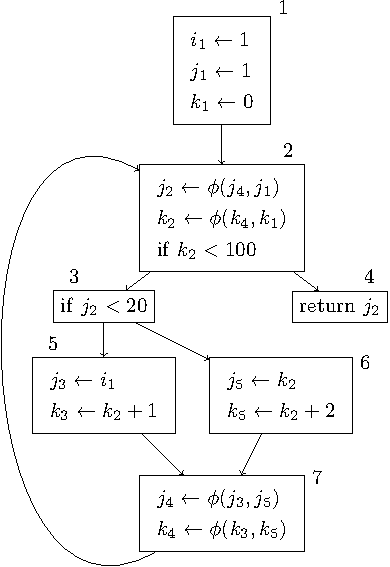
\includegraphics[width=.3\textwidth]{SSA-prog-crop.pdf}
     }
     &
     {\small
     \begin{tabularx}{0.3\textwidth}{XXXXX}
       $B$ & $\mathcal{E}[B]$ & & $x$ & $\mathcal{V}[x]$\\\cline{1-2}\cline{4-5}
       1 & $true$ & & $i_1$ & $1$\\
       2 & $true$ & & $j_1$ & $1$\\
       3 & $true$ & & $j_2$ & $1$\\
       4 & $true$ & & $j_3$ & $1$\\
       5 & $true$ & & $j_4$ & $1$\\
       6 & $false$ & & $j_5$ & $\bot$\\
       7 & $true$ & & $k_1$ & $0$\\
         &        & & $k_2$ & $\top$\\
         &        & & $k_3$ & $\top$\\
         &        & & $k_4$ & $\top$\\
         &        & & $k_5$ & $\bot$
     \end{tabularx}}
   \end{tabularx}
   \end{center}
   \greentext{$j$は定数が伝播して，$j<20$の判定がいつも成立．$k$は$\top$なので$k<100$の
   判定は実行時}
\end{frame}

\begin{frame}
  \frametitle{条件付き定数伝播}
  \begin{center}
    \only<1>{\greentext{定数の伝播と実行不可能な分岐の除去}}
    \only<2>{\greentext{単一引数のφ関数と不要なブロックの除去}}
    \begin{tabularx}{0.8\textwidth}{XXX}
      \multicolumn{1}{m{.3\textwidth}}{
        \only<1>{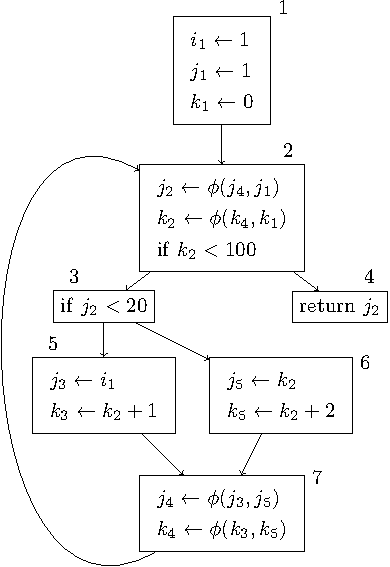
\includegraphics[width=.3\textwidth]{SSA-prog-crop.pdf}}
        \only<2>{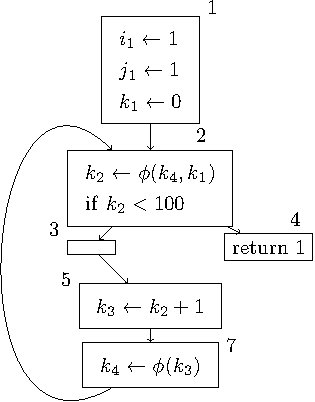
\includegraphics[width=.3\textwidth]{SSA-prog-opt1-crop.pdf}}
      }
      &
      \multicolumn{1}{m{2em}}{$\Rightarrow$} 
      &
      \multicolumn{1}{m{.3\textwidth}}
      {
        \only<1>{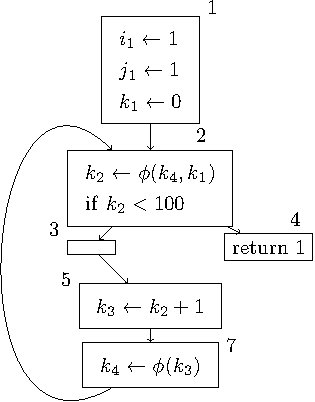
\includegraphics[width=.3\textwidth]{SSA-prog-opt1-crop.pdf}}
        \only<2>{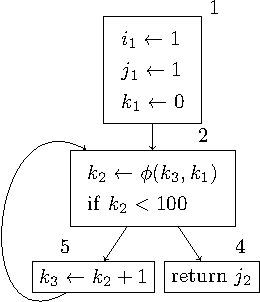
\includegraphics[width=.3\textwidth]{SSA-prog-opt2-crop.pdf}}
      }
    \end{tabularx}
  \end{center}
\end{frame}

\subsection{逆変換アルゴリズム}

\begin{frame}
  \frametitle{逆変換アルゴリズム}

    先行ブロックにフローごとの
    先行ブロックの最後がgoto文の場合は、goto文の直前に代入文を挿
    入する。
  
    \only<1>{
        \begin{center}


    \begin{tabular}{cc}
        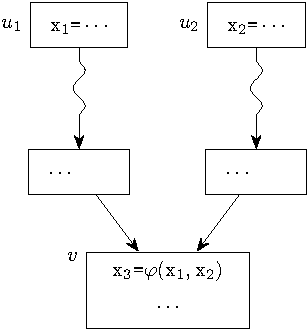
\includegraphics[width=.3\linewidth]{SSA-phiElimination-a-crop.pdf}
         &
        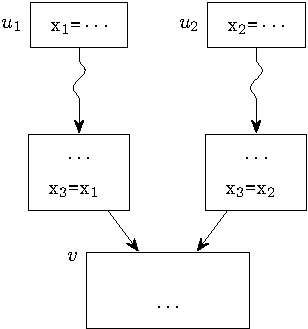
\includegraphics[width=.3\linewidth]{SSA-phiElimination-b-crop.pdf}
    \end{tabular}
\end{center}
    }

    \only<2>{

  \begin{trivlist}
    \item [1.] フローグラフの変換\\
    $\phi$関数を持つブロックに対して挿入条件を満たさないまで、代
    入文を挿入する。

    \vspace*{1zw}

    挿入条件：$\phi$関数を持つブロックが複数の先行頂点を持ち、そ
    のうちの一つが複数の後続頂点を持つ。

    \vspace*{1zw}

    \item [2.] $\phi$関数の消去
  \end{trivlist}
    }
\end{frame}



\begin{frame}
  \frametitle{逆変換例}

  %\greentext{(p.136 演習問題3)}

  \only<1>{
    \begin{center}
      \scalebox{0.75}{
        \begin{tikzpicture}
          \node[anchor=west,draw,minimum width=3.8cm] (v0) at (0,6.5)
          {\small $\begin{array}{ll}\hspace*{1zw}
                 & \mathtt{i_1=1}                              \\[-2pt]
                 & \mathtt{j_1=1}                              \\[-2pt]
                 & \mathtt{k_1=1}                              \\[-2pt]
                 & \mathtt{if}\ p'\ \mathtt{goto}\ \mathtt{L1} \\\end{array}$};
          \node at ($(v0)+(-2.2,0.7)$) {$v_0$};
          \node[anchor=west,draw,minimum width=3.8cm] (v1) at (0,4.25)
          {\small $\begin{array}{ll}
                L3: & \mathtt{i_2=}\phi\mathtt{(i_1,i_3)}        \\[-2pt]
                    & \mathtt{if}\ q\ \mathtt{goto}\ \mathtt{L2} \\
              \end{array}$};
          \node at ($(v1)+(-2.2,0)$) {$v_1$};
          \node[anchor=west,draw,minimum width=3.8cm] (v2) at (0,2.5)
          {\small $\begin{array}{ll}
                \hspace*{1zw} & \mathtt{i_3=i_2+1} \\
                              & \mathtt{goto\ L3}
              \end{array}$};
          \node at ($(v2)+(-2.2,0.2)$) {$v_2$};
          \node[anchor=west,draw,minimum width=3.8cm] (v3) at (0,1)
          {\small $\begin{array}{ll}
                L1: & \mathtt{j_2=i_1+k_1} \\
              \end{array}$};
          \node at ($(v3)+(-2.2,0)$) {$v_3$};
          \node[anchor=west,draw,minimum width=3.8cm] (v4) at (0,-0.5)
          {\small $\begin{array}{ll}
                L2: & \mathtt{i_4=}\phi\mathtt{(i_2,i_1)} \\
                    & \mathtt{j_3=}\phi\mathtt{(j_1,j_2)} \\
                    & \mathtt{k_2=i_4+j_3}                \\
              \end{array}$};
          \node at ($(v4)+(-2.2,0)$) {$v_4$};
          \path[->] (v0) edge (v1);
          \path[->] (v1) edge (v2);
          \path[->] (v2) [out=210,in=150,looseness=3] edge (v1);
          \path[->] (v0) [out=350,in=10,looseness=0.5] edge (v3);
          \path[->] (v1) [out=350,in=10,looseness=0.5] edge (v4);
          \path[->] (v3) edge (v4);
        \end{tikzpicture}
      }
    \end{center}
  }
  \only<2>{
    \scalebox{0.8}{
      \begin{tikzpicture}
        \node[anchor=west,draw,minimum width=3.8cm] (v0) at (0,6.5)
        {\small $\begin{array}{ll}\hspace*{1zw}
               & \mathtt{i_1=1}                              \\[-2pt]
               & \mathtt{j_1=1}                              \\[-2pt]
               & \mathtt{k_1=1}                              \\[-2pt]
               & \mathtt{if}\ p'\ \mathtt{goto}\ \mathtt{L1} \\\end{array}$};
        \node at ($(v0)+(-2.2,0.7)$) {$v_0$};
        \node[anchor=west,draw, minimum width=3.8cm,minimum height=5mm,fill=lightlightgrey] (w0) at (0,5)
        {$\hspace*{1zw}\mathtt{i_2=i_1}$};
        \node at ($(w0)+(-2.2,0)$) {$w_0$};
        \node[anchor=west,draw,minimum width=3.8cm] (v1) at (0,3.8)
        {$\mathtt{L3:\ if}\ q'\ \mathtt{goto}\ \mathtt{L2}$};
        \node at ($(v1)+(-2.2,0)$) {$v_1$};
        \node[anchor=west,draw,minimum width=3.8cm] (v2) at (0,2)
        {$\begin{array}{ll}\hspace*{1zw} & \mathtt{i_3=i_2+1} \\[-2pt]
                               & \mathtt{i_2=i_3}   \\[-2pt]
                               & goto\ L3\end{array}$};
        \node at ($(v2)+(-2.2,0.6)$) {$v_2$};
        \node[anchor=west,draw,minimum width=3cm,minimum height=8mm,fill=lightlightgrey] (w1) at (5,2)
        {$\begin{array}{ll}L2: & \mathtt{i_4=i_2} \\[-2pt] & \mathtt{j_3=j_1}\\[-2pt]
                     & goto\ L4
            \end{array}$};
        \node at ($(w1)+(-1.8,0.3)$) {$w_1$};
        \node[anchor=west,draw,minimum width=3.8cm] (v3) at (9,4)
        {$\begin{array}{ll}L1: & \mathtt{j_2=i_1+k_1} \\
                     & \mathtt{i_4=j_1}     \\ & \mathtt{j_3=j_2}\end{array}$};
        \node at ($(v3)+(-2.2,0.4)$) {$v_3$};
        \node[anchor=west,draw,minimum width=3.8cm] (v4) at (9,0)
        {$L4:$\ $\mathtt{k_2=i_4+j_3}$};
        \node at ($(v4)+(-2.2,0)$) {$v_4$};
        \path[->] (v0) edge (w0)  (w0) edge (v1)  (v1) edge (v2)  (v2) [out=190,in=170,looseness=1] edge (v1);
        \path[->] (v1) [out=350,in=135] edge (w1)  (w1) [out=330,in=120] edge (v4);
        \path[->] (v3) edge (v4);
        \path[->] (v0) [out=330,in=135] edge (v3);
      \end{tikzpicture}
    }
  }
\end{frame}

\begin{frame}[fragile]
    \frametitle{$\varphi$関数のないSSA形式}
    \begin{center}
    \begin{minipage}{.3\linewidth}
    \begin{Verbatim}[fontsize=\small,frame=single,xrightmargin=-5mm]
    i1 = 1
    j1 = 1
    k1 = 1
    if p' goto L1
    i2 = i1
L3: if q' goto L2
    i3 = i2 + 1
    i2 = i3
    goto L3
L2: i4 = i2
    j3 = j1
    goto L4
L1: j2 = i1 + k1
    i4 = j1
    j3 = j2
L4: k2 = i4 + j3
    \end{Verbatim}
\end{minipage}
\end{center}
\end{frame}
\end{document}